\documentclass{standalone}
\usepackage{tikz}
\usetikzlibrary{shapes,arrows.meta}
\begin{document}
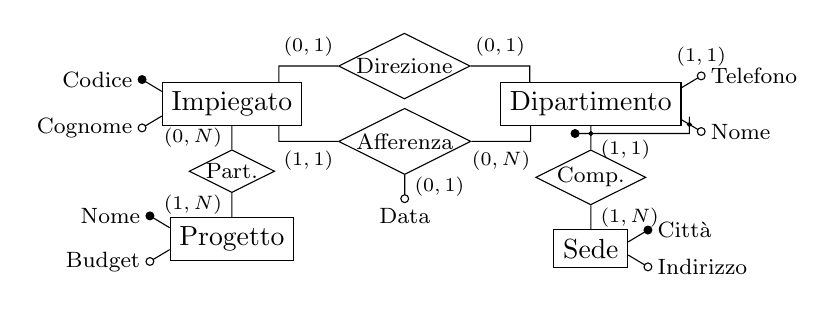
\begin{tikzpicture}
    \draw

    %%* Attributi:
    %%  node[draw, circle, inner sep=1pt, fill=black]{}node[right]{\footnotesize A}
    %%? Distanza orizzontale: E -(0.25,0.x)- A
    %%? Distanza verticale: E -(0,x * 0.22)- A

    %%* Cardinalità:
    %%  node[below right]{\scriptsize $(0,N)$}
    %%  node[above right]{\scriptsize $(0,N)$}
    %%  node[midway, above]{\scriptsize $(0,N)$}

    %%* Relazione:
    %%  node[draw, diamond, shape aspect=2, inner sep=3pt, anchor=90](r1){}
    %%  node[draw, diamond, shape aspect=2, inner sep=0.2pt, anchor=180](r2){R2}

    %%* Entità:
    %%  node[draw, rectangle, anchor=90](e1){}
    %%? Distanza verticale: E -(0.3)- R -(0.3) E
    %%? Distanza orizzontale: E -(0.75)- R -(0.75)- E

    %%* Impiegato
    (0,0)node[draw, rectangle, anchor=90](imp){Impiegato}
    (imp.190)--++(-0.25,-0.15)node[draw, circle, inner sep=1pt, fill=white]{}node[left]{\footnotesize Cognome}
    (imp.170)--++(-0.25,0.15) node[draw, circle, inner sep=1pt, fill=black]{}node[left]{\footnotesize Codice}

    %%* Progetto
    (imp.270)--++(0,-0.3)node[midway, left]{\scriptsize $(0,N)$}node[draw, diamond, shape aspect=2, inner sep=0.2pt, anchor=90](r1){\footnotesize Part.}
    (r1.270)--++(0,-0.3) node[midway, left]{\scriptsize $(1,N)$}node[draw, rectangle, anchor=90](prg){Progetto}
    (prg.190)--++(-0.25,-0.15)node[draw, circle, inner sep=1pt, fill=white]{}node[left]{\footnotesize Budget}
    (prg.170)--++(-0.25,0.15) node[draw, circle, inner sep=1pt, fill=black]{}node[left]{\footnotesize Nome}

    %%* Afferenza
    (imp.335)--++(0,-0.2)--++(0.75,0)node[midway, below]{\scriptsize $(1,1)$}node[draw, diamond, shape aspect=2, inner sep=0.3pt, anchor=180](r2){\footnotesize Afferenza}
    (r2.0)   --++(0.75,0) node[midway, below]{\scriptsize $(0,N)$}--++(0,0.2)node[draw, rectangle, anchor=200](dip){Dipartimento}
    (r2.270) --++(0,-0.3)node[draw, circle, inner sep=1pt, fill=white]{}node[below]{\footnotesize Data}node[midway, right]{\scriptsize $(0,1)$}
    %%* Direzione
    (imp.25)--++(0,0.2) --++(0.75,0)node[midway, above]{\scriptsize $(0,1)$}node[draw, diamond, shape aspect=2, inner sep=0.3pt, anchor=180](r2){\footnotesize Direzione}
    (r2.0)  --++(0.75,0)node[midway, above]{\scriptsize $(0,1)$}--++(0,-0.2)

    %%* Dipartimento
    (dip.270)--++(0,-0.1)node[draw, circle, inner sep=0.5pt, fill=black](a){}--++(0,-0.2)node[right]{\scriptsize $(1,1)$}node[draw, diamond, shape aspect=2, inner sep=0.2pt, anchor=90](r1){\footnotesize Comp.}
    (dip.350)--++(0.1,-0.06)node[draw, circle, inner sep=0.5pt, fill=black](b){}--++(0.15,-0.09)node[draw, circle, inner sep=1pt, fill=white]{}node[right]{\footnotesize Nome}
    (dip.10)--++(0.25,0.15)node[above]{\scriptsize $(1,1)$}node[draw, circle, inner sep=1pt, fill=white]{}node[right]{\footnotesize Telefono}
    (a)--++(-0.2,0)node[draw, circle, inner sep=1pt, fill=black]{}-|(b)--++(0,0.1)

    %%* Sede
    (r1.270)--++(0,-0.3)node[midway, right]{\scriptsize $(1,N)$}node[draw, rectangle, anchor=90](prg){Sede}
    (prg.350)--++(0.25,-0.15)node[draw, circle, inner sep=1pt, fill=white]{}node[right]{\footnotesize Indirizzo}
    (prg.10)--++(0.25,0.15)node[draw, circle, inner sep=1pt, fill=black]{}node[right]{\footnotesize Città}
    

    ;
\end{tikzpicture}
\end{document}